\documentclass[a4paper,12pt]{article}
\usepackage{fancyhdr}
\usepackage{lastpage}
\usepackage{geometry}
\usepackage{listings}
\usepackage{datetime}
\usepackage{xeCJK}
\usepackage{hyperref}
\usepackage{amsmath}
\usepackage{graphicx}
\usepackage{float} % 加入 float 宏包以使用 [H]
\usepackage{longtable}

\geometry{left=2.5cm, right=2.5cm, top=2.5cm, bottom=2.5cm}
\pagestyle{fancy}
\setCJKmainfont{Noto Sans CJK HK}
% 英文字體 consolas
\setmonofont{Consolas}
% 設定內文文字大小
\renewcommand{\normalsize}{\fontsize{12pt}{\baselineskip}\selectfont}

% 設定頁首
\fancyhf{}
\fancyhead[L]{Volume Rendering and Gradient Visualization}
\fancyhead[R]{\today}
\fancyfoot[C]{\thepage/\pageref{LastPage}}

\title{Volume Rendering and Gradient Visualization}
\author{01057033洪銘均}
\date{\today}

\begin{document}
\maketitle
\tableofcontents
\newpage

\section{程式概述}
該程式使用imgui搭配資料處理與統計的方式,在預處理時利用CDF均衡化統計資料不平衡,再計算梯度後利用imgui做梯度與統計數據的視覺化



\section{運行結果}

\begin{figure}[h]
    \centering
    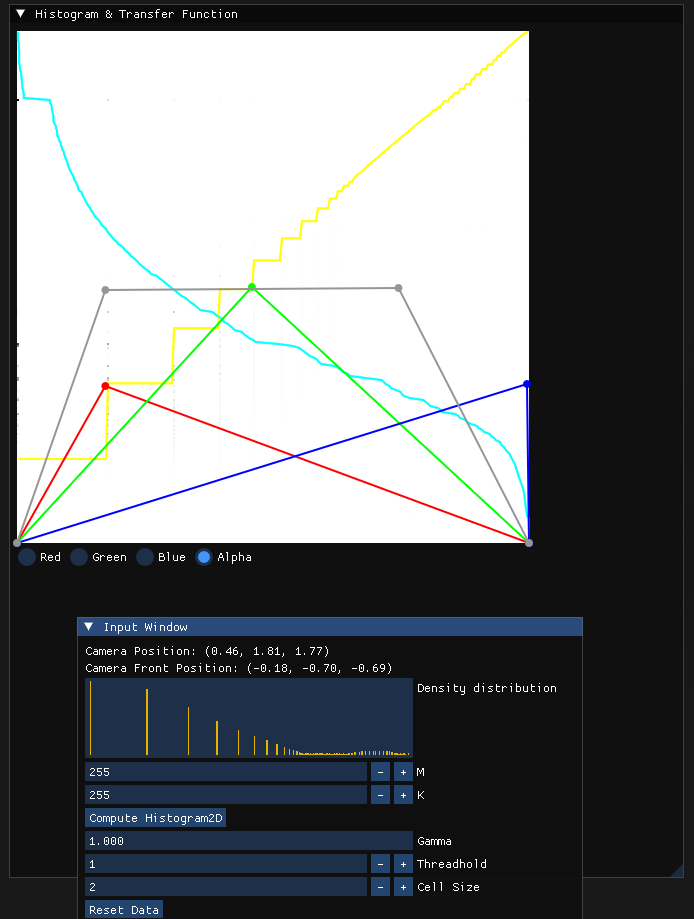
\includegraphics[width=0.8\textwidth]{img/img2.png}
\end{figure}
圖中縱軸為梯度值、橫軸為密度值,黃色為密度值累積、青色為梯度值累積,可以看到利用CDF映射後成功讓資料分散化,並且

\section{心得}
這次得作業實做牛頓2D的計算過程,牛頓法在上課時聽得沒很懂,也是到時做前才搞懂流程。在實做中利用到矩陣運算庫Eigen來完成部份矩陣操作包含反矩陣、矩陣乘法等。在視覺化上,我利用GLSL差值來完成函數和收斂點過程圖形的繪製,雖然一開始遇到線條粗細不一,特定情況下還會出現函數扭曲,但後來加上fwidth就成功修正這問題了。
在後續也嘗試不同的函數來觀察收斂過程,雖然在過程中出現與預期收斂結果不同的情況,在偵錯過程中發現偏微分計算結果有問題,持續追查才發現是我函數初始格式錯誤,後續解決後也正常執行了。

\end{document}

% xelatex  --max-print-line=10000 -synctex=1 -interaction=nonstopmode -file-line-error -recorder .\codebook.tex 
